\documentclass[../main.tex]{subfiles}
\graphicspath{{\subfix{../diagrams/}}}

\begin{document}

\section{AlexCore}
Add text here


\subsection{Core Architecture and Pipelines}
AlexCore has five stages; frontend, decode, issue, execute, and commit. Each stage has one pipeline except for the frontend and execute stages each having two pipelines, making a total of seven pipelines.

\subsubsection{Stage details}
\begin{enumerate}
  \item \textbf{Frontend:} \\
  Fetches instructions from memory via the OpenPiton core interface, capable of fetching one instruction per cycle.
 \item \textbf{Decode:}\\
 Decodes fetched instruction and sets control signals accordingly. 
 \item \textbf{Issue:}\\
 Register file and CSR  read and write operations all occur in this stage. This stage also includes the scoreboard, which manages data, control, and memory hazards.\\ The frontend, decode, and issue stages are stalled on hazards.
 \item \textbf{Execute:}\\
This stage includes the ALU, multiplication and division unit, memory controller, CSR unit, exceptions logic, and write-back multiplexer.
 \item \textbf{Commit:}\\
 Contains the write back values to the register file and CSR register file. 
\end{enumerate}

\begin{figure}[bh]
\centering
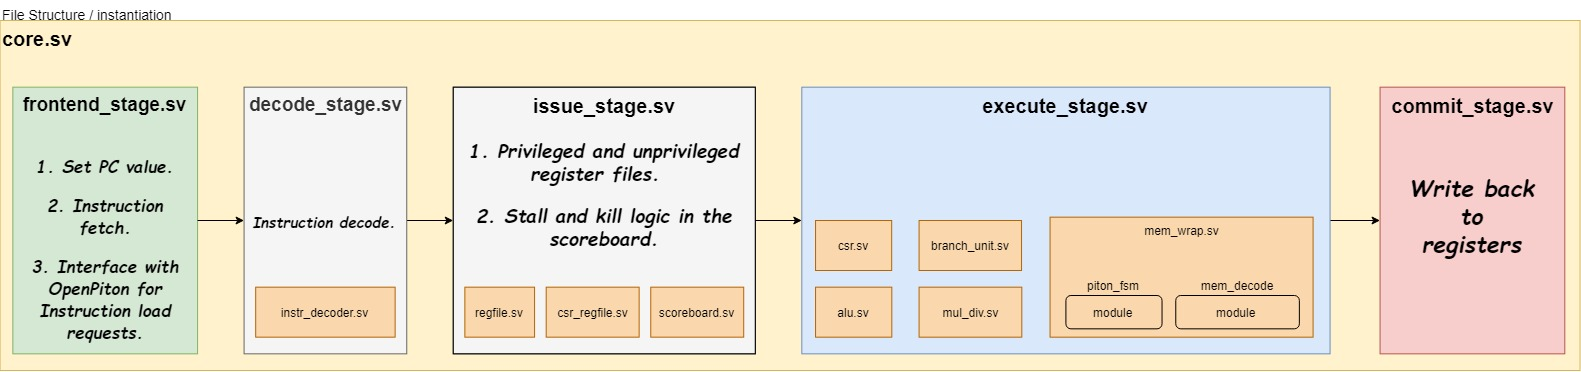
\includegraphics[width=15cm, height=7cm]{diagrams/CoreHirearchy.jpg}

\caption{Core file hirearchy}
\label{fig:files}
\end{figure}

\begin{figure}[p]
\centering
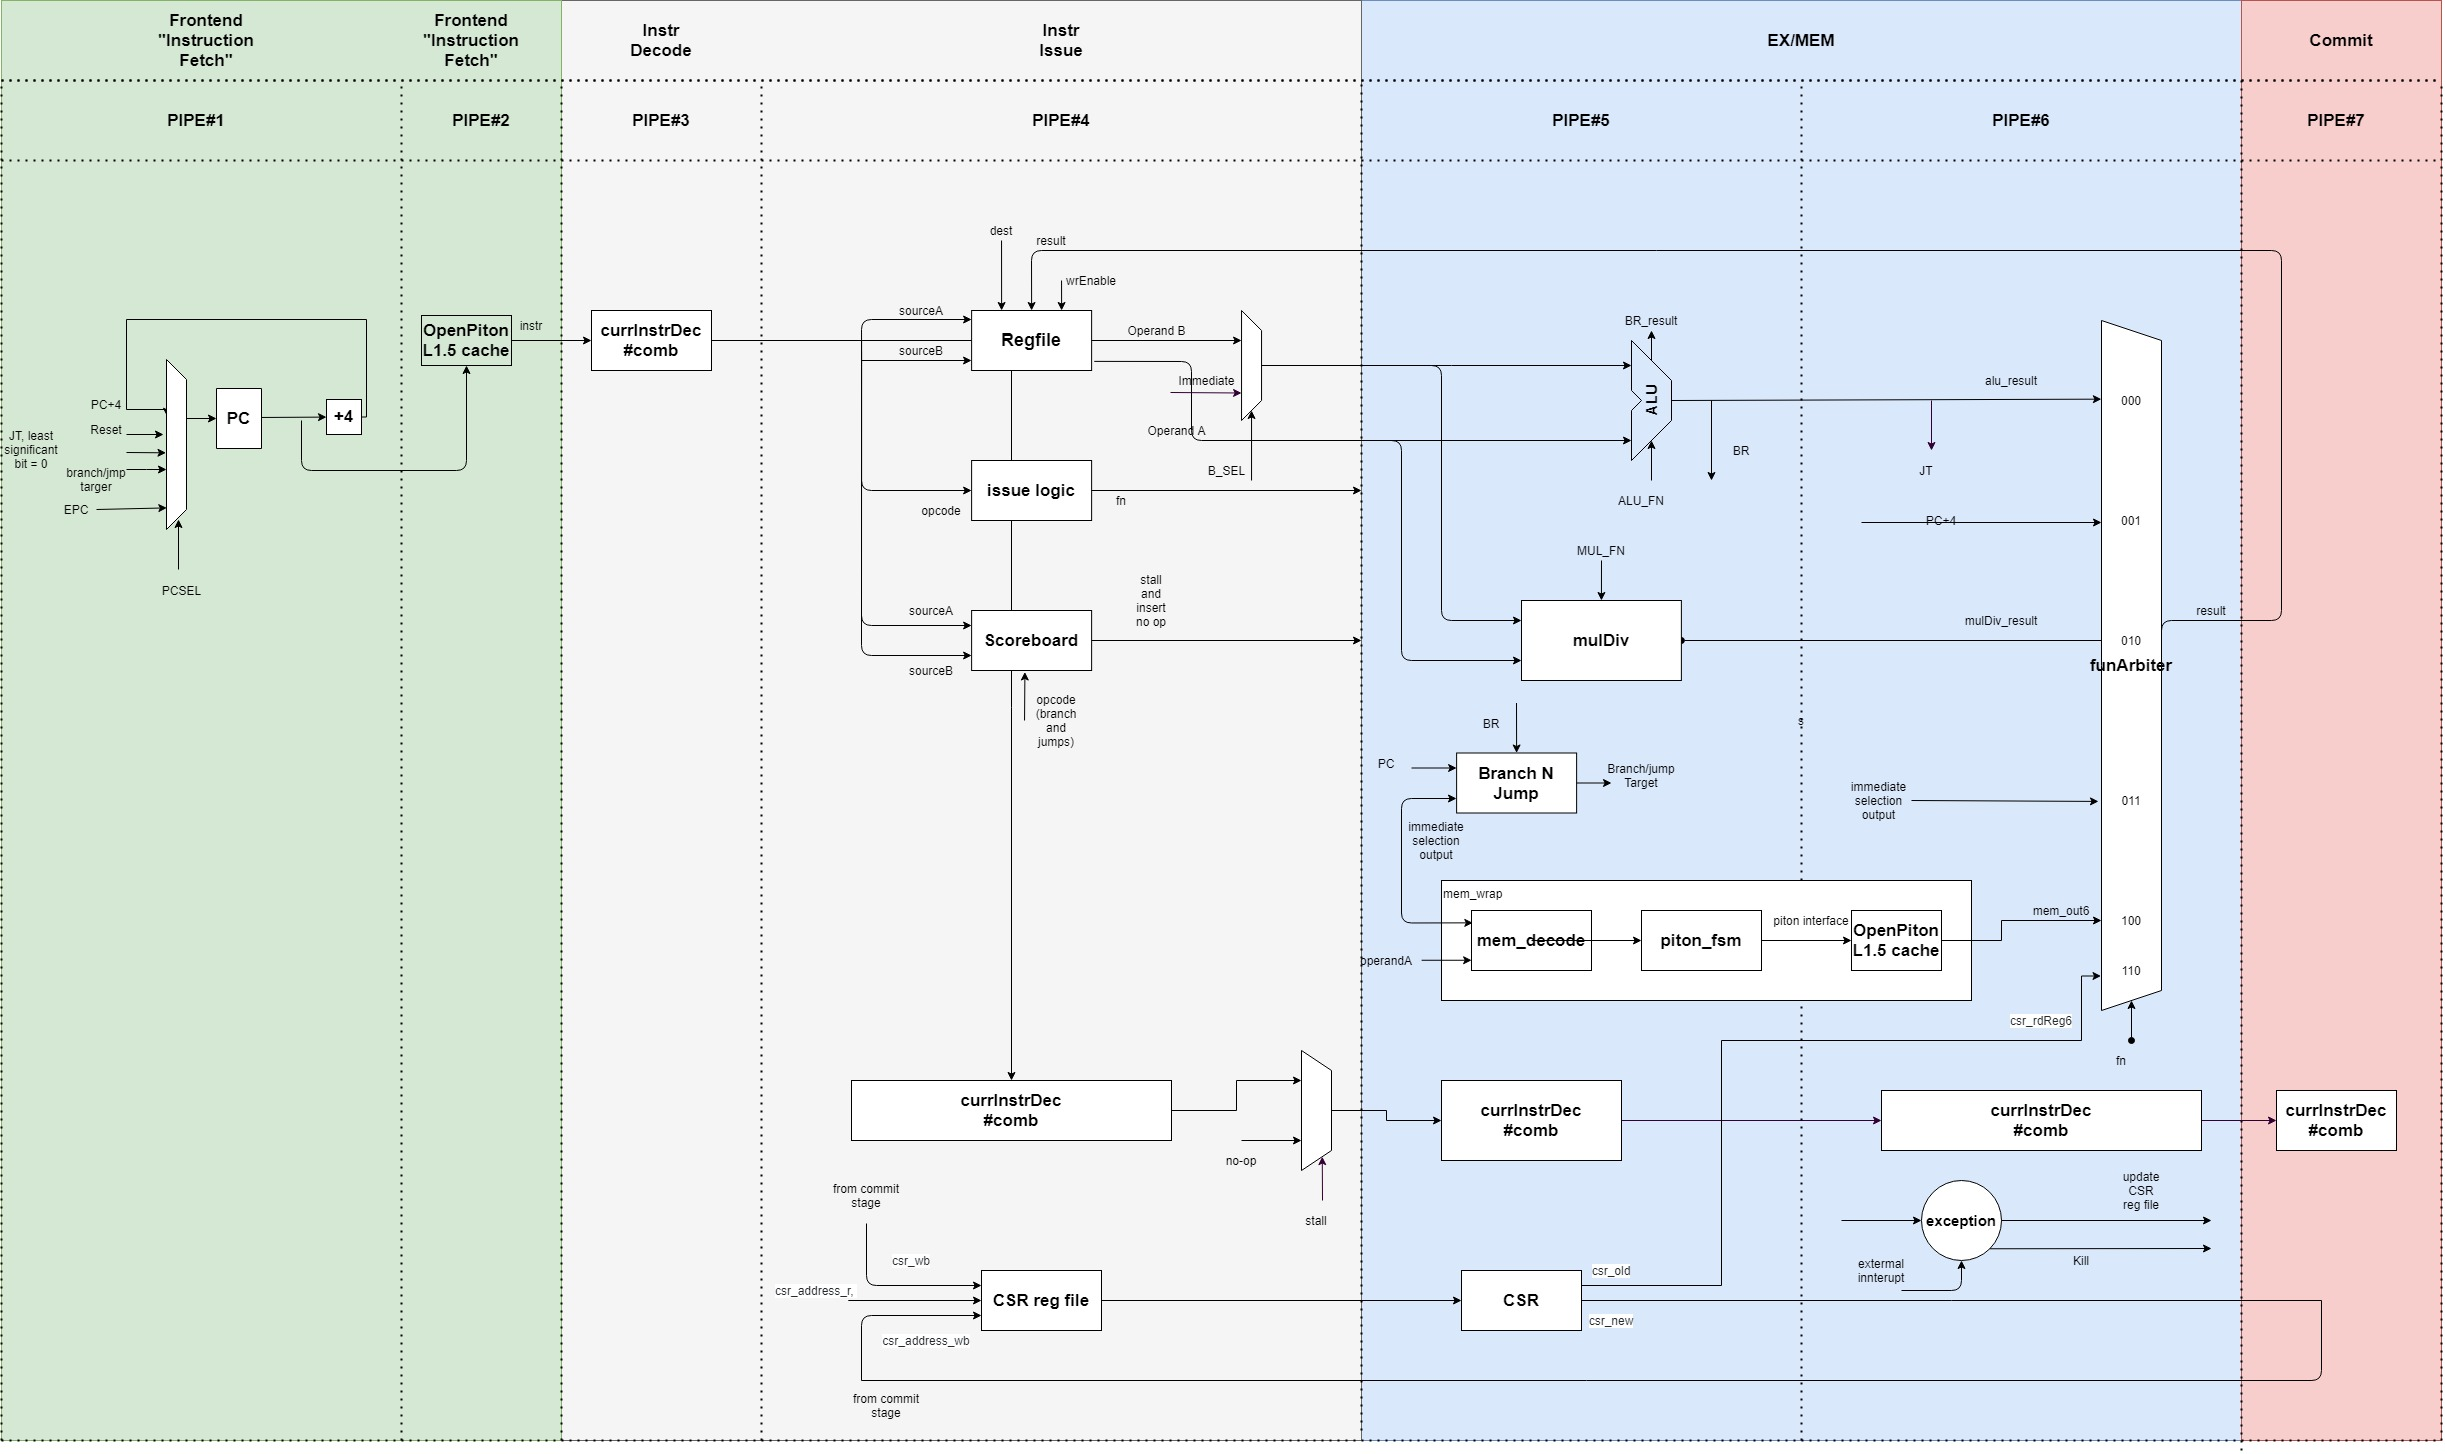
\includegraphics[scale = 0.27,angle = 90]{diagrams/CoreTopLevel.jpg}

\caption{Core Architecture Diagram}
\label{fig:img1}
\end{figure}

\subsection{Arithmetic and Logic Operations}
The execution of these operations is split between two units; ALU, and multiplication and division unit. The ALU executes I-extension operations while the multiplication and division unit executes M-extension operations. The ALU also performs calculation regarding branch operations.

\subsubsection{ALU operations}
The ALU takes the following input signals:
\begin{itemize}
  \item alu\_fn: selects the operation that the ALU will perform.
  Table \ref{ch4.1} shows the input values corresponding to each operation 
   \item btype: determines that the ALU operation is a branch operation. 
   \item bneq: asserts the branch signal if operandA and operandB are not equal.
  \item operandA: ALU input A.
  \item operandB: ALU input B.
\end{itemize}

\noindent The ALU takes the following output signals:
\begin{itemize}
  \item btaken: Indicates that the branching condition is met.
  \item result: ALU arithmetic and logical operation result output.
\end{itemize}

\begin{table}[h!]
\begin{center}
\begin{tabular}{|c | c|}
    \hline
    alu\_fn & Mnemonic\\
    \hline
    4'b0001 & ADDI, ADD  \\ 
    \hline
	4'b0001 & SLLI, SLL  \\
	\hline
	4'b0010 & SLTI, SLT  \\
	\hline
	4'b0011 & SLTIU, SLTU \\
	\hline
	4'b0100 & XORI, XOR  \\
	\hline
	4'b0101 & SRLI, SRL  \\
	\hline
	4'b0110 & OR, ORI \\ 
	\hline
	4'b0111 & ANDI, AND \\
	\hline
	4'b1000 & SUB \\
	\hline
	4'b1001 & BGE\\  
	\hline
	4'b1010 & BGEU \\ 
	\hline
	4'b1101 & SRAI, SRA \\
	\hline
\end{tabular}
\end{center}
\caption{ALU operations}
\label{ch4.1}
\end{table}

\subsubsection{Multiplication and division operations}
It takes the following input signals:
\begin{itemize}
   \item  mulDiv\_op: selects the operation type. Table \ref{ch4.2} shows the input values corresponding to each operation
   \item a,b: input operands.
\end{itemize}

And res as the output result signal.

\begin{table}[h!]
\begin{center}
\begin{tabular}{|c | c|}
    \hline
    mulDiv\_op & Mnemonic\\
    \hline
    4'b0000 & NoOp  \\ 
    \hline
	4'b0011 & MUL  \\
	\hline
	4'b0101 & MULH  \\
	\hline
	4'b0111 & MULHU \\
	\hline
	4'b0110 & MULHSU  \\
	\hline
	4'b1001 & DIV  \\
	\hline
	4'b1011 & DIVU \\ 
	\hline
	4'b1101 & REM \\
	\hline
	4'b1111 & REMU \\
	\hline
\end{tabular}
\end{center}
\caption{Multiply/divide operations}
\label{ch4.2}
\end{table}

%%%%%%%%%%%%%%%%%%%%%%%%%%%%%%%%%%%%%%%%%%%%%%%%%%%%%%%%%%%%%%%%%
\subsection{Handling Hazards}
\begin{enumerate}
\item \textbf{Introduction}\\
In the domain of central processing unit (CPU) design,hazards are problems with the instruction pipeline in CPU micro architectures when the next instruction cannot execute in the following clock cycle, and can potentially lead to incorrect computation results. Three common types of hazards are data hazards, structural hazards, and control hazards (branching hazards),all these hazards depend on the architecture of the design so it is not a must to deal with all of them.

There are several methods used to deal with hazards, including pipeline stalls/pipeline bubbling, operand forwarding, and in the case of out-of-order execution, the scoreboarding method.
The problem is you want run sequential commands but in a parallel form to maximize your hardware usage so the synchronization is handled in this part.

\item \textbf{Hazard types}

\begin{itemize}
     \item \textbf{data Hazards}\\

        Data hazards occur when instructions that exhibit data dependence modify data in different stages of a pipeline. Ignoring potential data hazards can result in race conditions (also termed race hazards). There are three situations in which a data hazard can occur and it depend on the architecture of the design.\\
        
   \begin{figure}[bh]
\centering
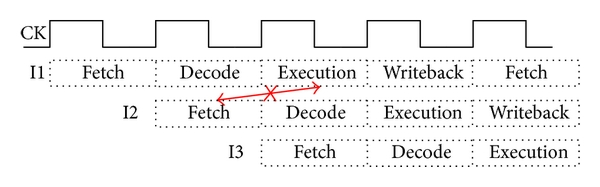
\includegraphics[scale=2]{diagrams/hazardcondition.jpg}

\caption{Hazard condition}
\label{fig:img}
\end{figure}\cleardoublepage
    
  

\noindent \textbf {Data hazards types}
\begin{itemize}
  \item    {Read after write (RAW)}\\


 {Example}\\
 


i1. R2 \textless-  R5 + R3\\
i2. R4 \textless- R2 + R3\\


\item  {Write after read (WAR)}\\


  {Example}\\


i1. R4 \textless- R1 + R5\\
i2. R5 \textless- R1 + R2\\


\item  {Write after write (WAW)}\\


 {Example}\\


i1. R2 \textless- R4 * R7\\
i2. R2 \textless- R1 + R3\\
\end{itemize}

 
     \item \textbf {structural hazards}\\
     A structural hazard occurs when two (or more) instructions that are already in pipeline need the same resource. The result is that instruction must be executed in series rather than parallel for a portion of pipeline. Structural hazards are sometime referred to as resource hazards.

Example: A situation in which multiple instructions are ready to enter the execute instruction phase and there is a single ALU (Arithmetic Logic Unit). One solution to such resource hazard is to increase available resources, such as having multiple ports into main memory and multiple ALU (Arithmetic Logic Unit) units.
     \item \textbf {control hazards}\\
     Control hazard occurs when the pipeline makes wrong decisions on branch prediction and therefore brings instructions into the pipeline that must subsequently be discarded. The term branch hazard also refers to a control hazard.
\end{itemize}

\item \textbf{Solving Hazards}
In our system we used scoreboard to solve hazard.
In a scoreboard, the data dependencies of every instruction are logged, tracked and strictly observed at all times. Instructions are released only when the scoreboard determines that there are no conflicts with previously issued ("in flight") instructions. If an instruction is stalled because it is unsafe to issue (or there are insufficient resources), the scoreboard monitors the flow of executing instructions until all dependencies have been resolved before the stalled instruction is issued.
So we mainly track every instructions and stall if it will cause hazard problem.\\
\\* \textbf {Stall uses in our design}
\begin{enumerate}
    \item using stall in  data dependencies mentioned like RAW,WAR and WAW.\\
    text here
    \item using stall to solve control hazards.\\
        text here

    \item using stall while switching between data memory and code memory.\\
        text here

    \item using stall if there is an AES custom instruction.\\
       text here

\end{enumerate}


\end{enumerate}
%%%%%%%%%%%%%%%%%%%%%%%%%%%%%%%%%%%%%%%%%%%%%%%%%%%%%%%%%%%%%%%%%


\end{document}
